\subsection{Written Communication\label{sec:written-communication}}

Reports, memos, emails are artifacts of bureaucracy in an organization. A written record creates evidence about policies and decisions. Existence of a record can be used for good or for harm.


% https://graphthinking.blogspot.com/2020/09/identifying-and-eliminating.html




%***************************

\subsubsection{Why written communication does not happen\label{sec:written-comm-does-not-happen}}
\begin{itemize}
    \item Too many reports/emails/memos/messages to read and process and respond to. Emotionally overwhelmed.
\item The person may read slowly.
\item The person may type slowly, or their hand writing is poor.
\item Fear of imperfect communication. What if the email is incomplete or inaccurate or ambiguous?
\item The person views written communication as ``official" or ``plan of record'' and does not feel comfortable brainstorming or creating contingency plans
\item The person wants to avoid accountability for their statements
\item The person may not be confident in their writing ability -- spelling, grammar, sentence composition, structuring content. \footnote{For tips on writing, see 
\href{https://en.wikipedia.org/wiki/The_Elements_of_Style}{The Elements of Style}
and
\href{https://www.google.com/search?q=dodm+5110.04}{DoDM 5110.04, Manual for Written Material}}
\end{itemize}



%***************************

\subsubsection{Email: A Piece of Art, A Form, and A Game\label{sec:}}

Originality is not a requirement in bureaucratic writing. Plagiarism is acceptable. The consistency of madlibs-based forms that follow decision trees is efficient. 

Readers need both context and conciseness. 

Using visual cues to improve readability

Email is a game of documenting decisions and responses so that the sequence of interactions is clear for audits and recrimination. 

\subsubsection{Email Responsiveness\label{sec:}}

three tiers of email responsiveness:
1) read all emails and reply to all emails
2) read all emails and reply to some
3) unable to read all incoming emails

The following scenarios are focused on case 2 -- able to triage (skim) emails but not enough time to respond to all.
****************************
Given insufficient time, which email do you reply to? An email from your boss, an email from your peer, an email from a person who reports to you, or a person who you do not know?
The ratio of these emails is not one to one to one to one.

1) the email from your boss is likely the top priority
of the remaining emails (peer, subordinate, unknown), 
2) peer is likely the next priority
3,4) the subordinate and unknown person are likely last

When there's insufficient time available, your transparency to subordinates and unknown people is likely to decrease

****************************
Three emails come in. One has no action, one is easy to reply to, and the third is difficult and takes time. Which one gets the response?
The ratio of these emails is not one to one to one.

1) the email that is easy to reply to gets answered first
2) the email that is difficult is second

If you only have time for one of the emails, it's likely to be the easy one. 
\href{https://en.wikipedia.org/wiki/Ambiguity_aversion}{ambiguity aversion}

As a consequence, outsiders see this as you are bike-shedding.
\href{https://en.wikipedia.org/wiki/Law_of_triviality}{law of triviality}

\subsection{Email Structure}

% from https://graphthinking.blogspot.com/2021/10/structuring-email-content-for.html

If implementing all these tips sounds like a lot of work, that's because it is. Effective written communication requires intentional effort because of the lack of augmenting channels (compared to voice or video or in-person). 



Use consistent design and structure for your emails. Emails are part of your professional reputation.

Emails start with a greeting: Hi, Hello, Good morning, Good afternoon, Good evening. 
Email greetings include the name of the targeted recipient(s). 

Emails terminate with a professional closing, e.g., "Kindly", "Regards", etc

Emails contain a signature block with contact information -- phone number, normal hours of response, which timezone you're in if your team spans timezones, how long to wait for a response before asking again, which communication channel I prefer, etc.

\begin{figure}
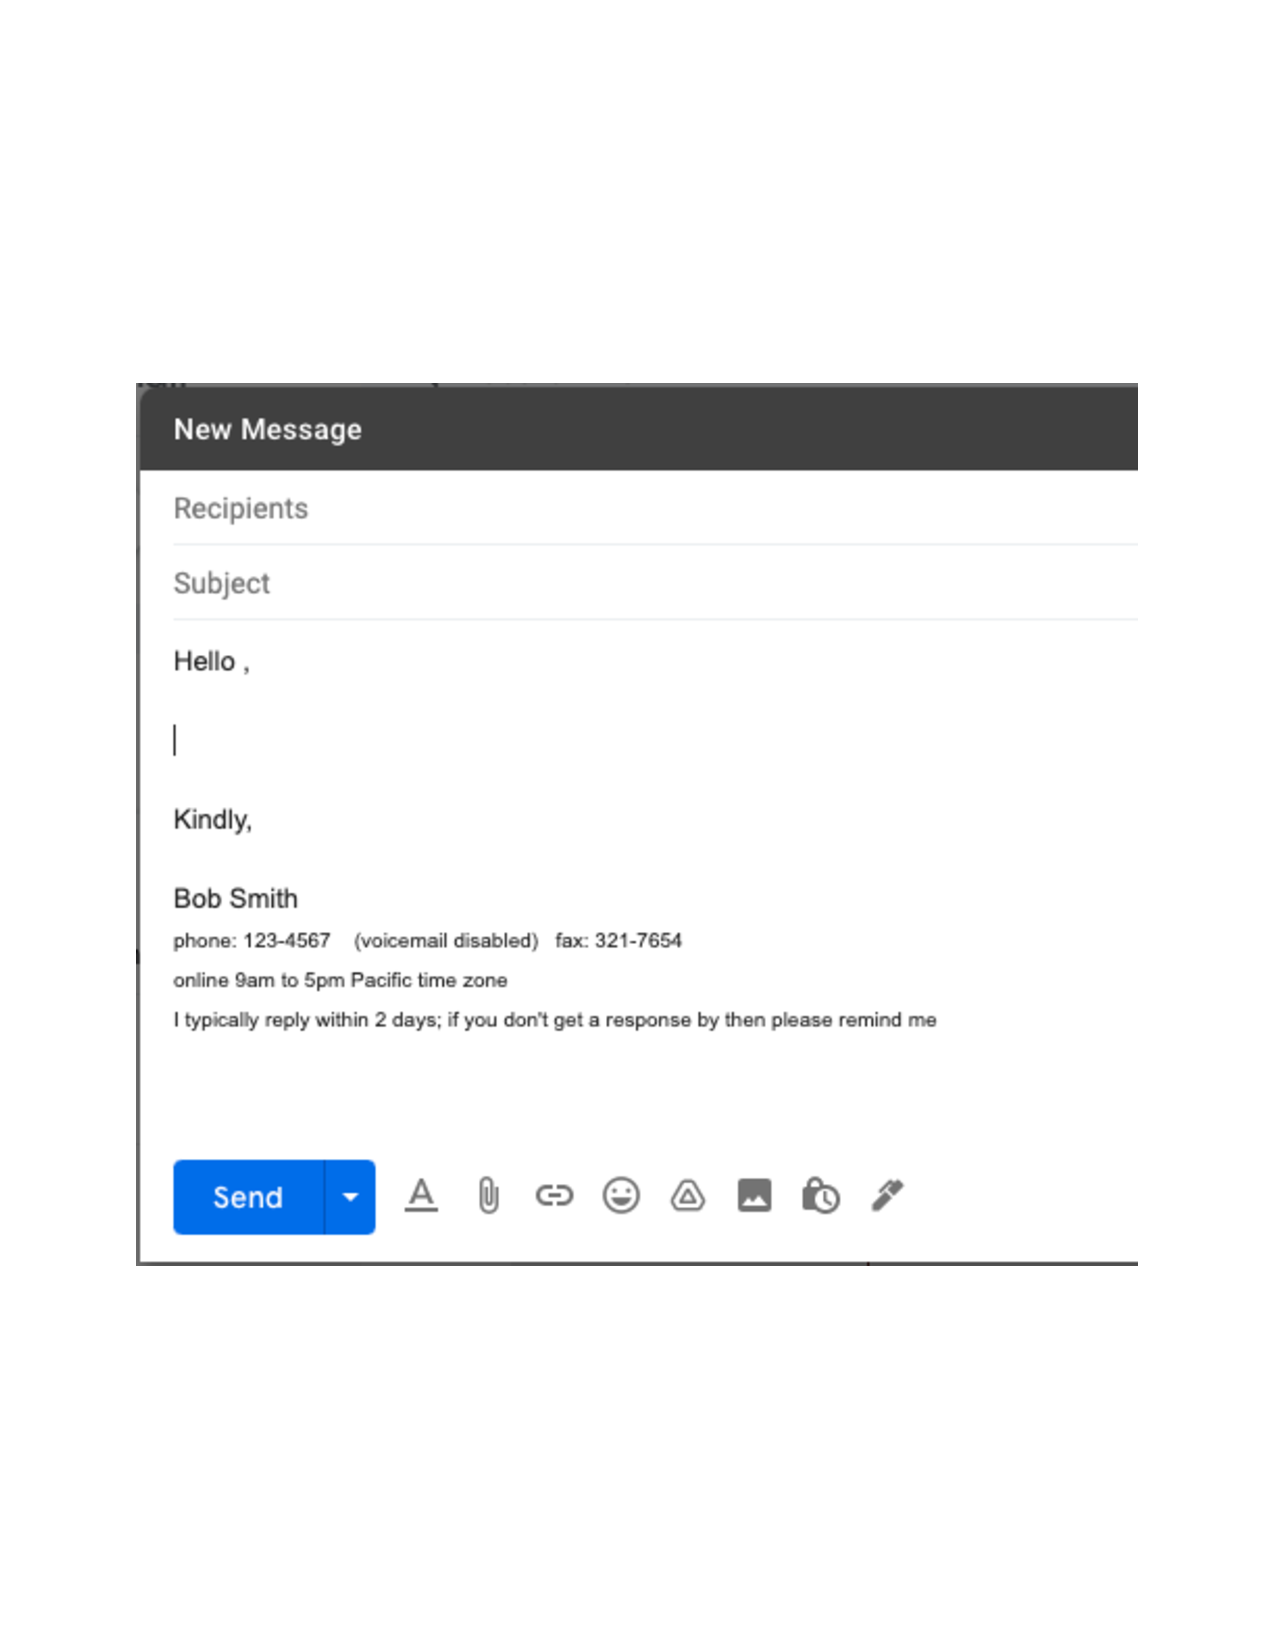
\includegraphics[width=1\textwidth]{images/email_template.pdf}
\caption{Template for new email messages. Greeting has a space after the comma -- that is where the recipient's name will go. Signature block uses smaller after the name.}
\label{fig:email_template}
\end{figure}

Email signature blocks do not include unnecessary images, as that uses more storage for recipients. 
Email threads focused on a specific instance of a recurring event include the date (YYYY-MM-DD) in the subject line. 

Based on the purpose of the email, example key phrases for subject lines include: "meeting notes" vs "agenda" vs "question about"

Revising an existing subject line can disrupt the ability of email software to thread conversations. However, sometimes the revision is worth breaking threading.

When replying to an ongoing thread, retain the original message as part of the thread to provide readers historical context.

When replying to threads with sensitive messages, sanitize the included content as appropriate by removing name or identifying details.

If an email contains multiple requests or questions, at the top of the email (after the greeting) explicitly say how many of each type. Then, in the body of the message, number them.

\begin{figure}
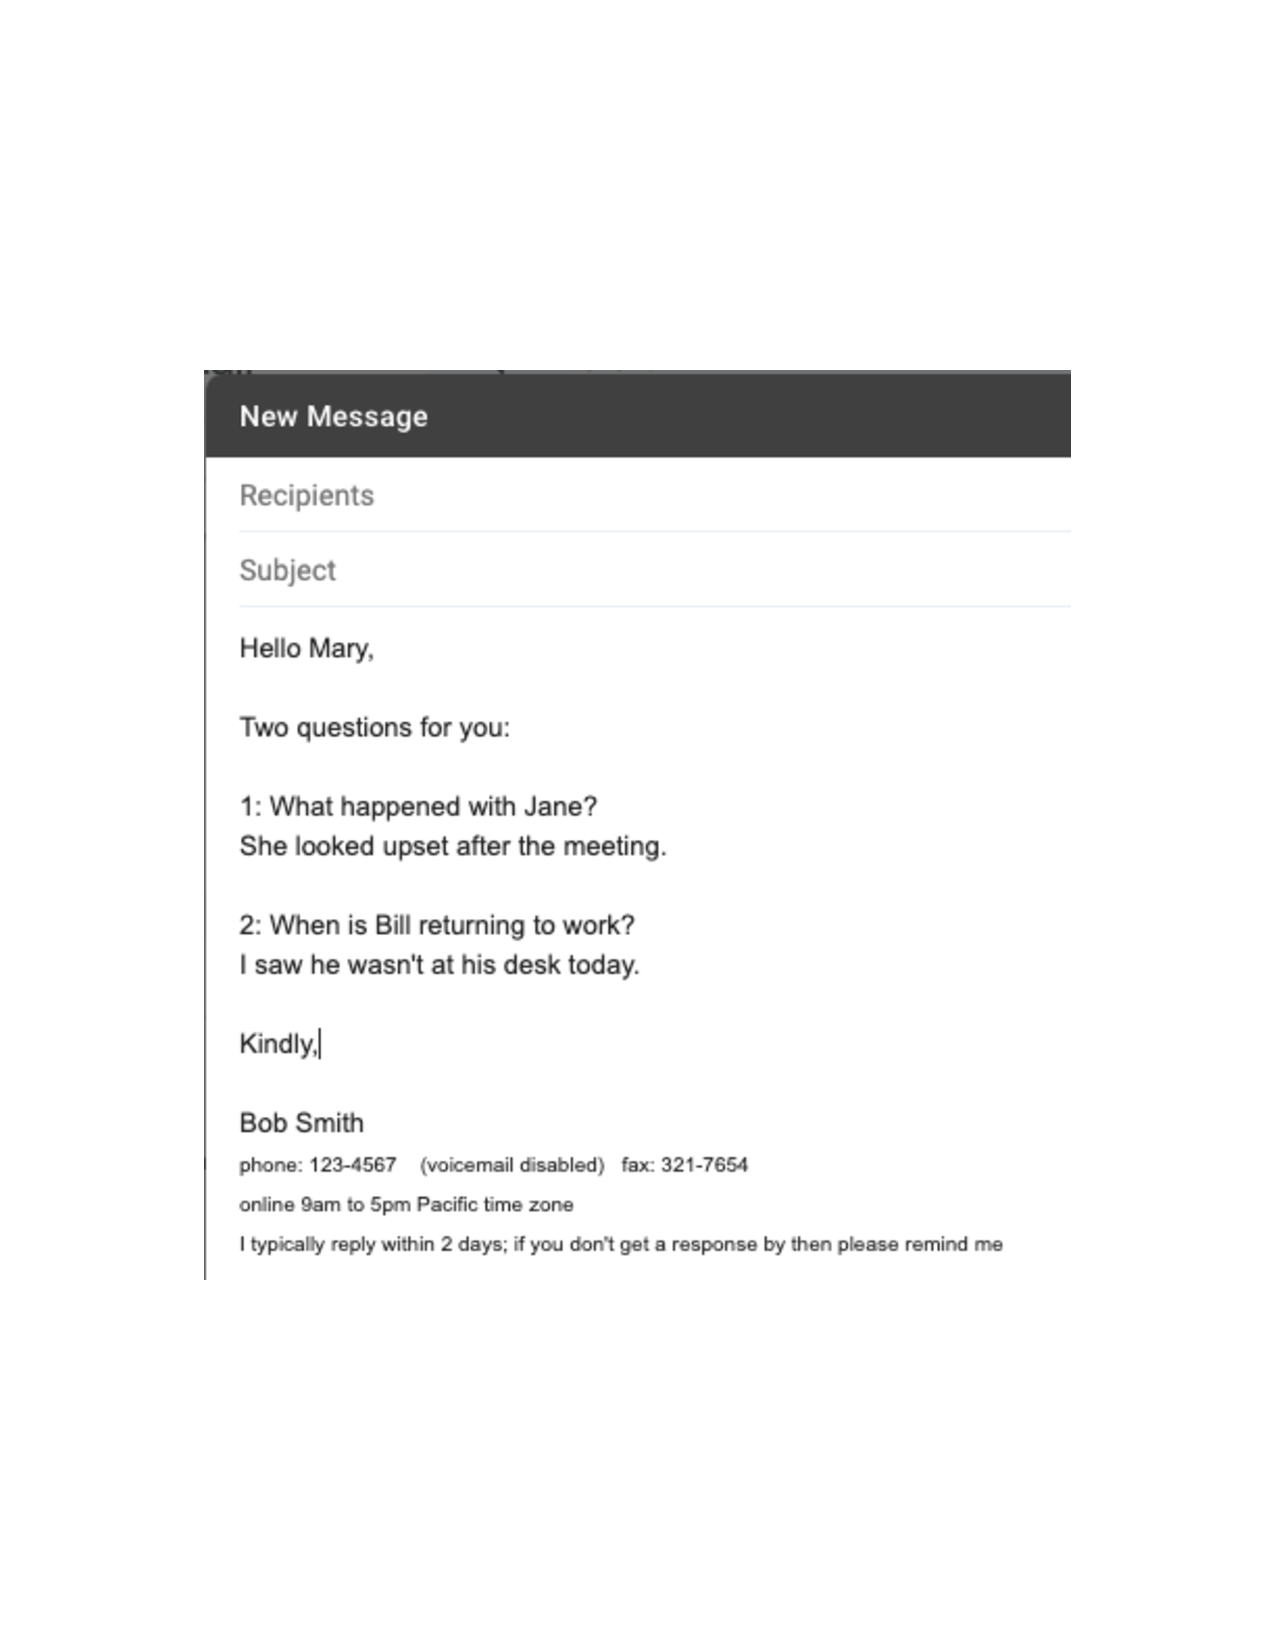
\includegraphics[width=1\textwidth]{images/email_two_questions.pdf}
\caption{Distinct items the recipient should address in a reply.}
\label{fig:email_two_questions}
\end{figure}

If an item corresponds to a requested action, separately highlight the action and indicate who is supposed to take the action and what the deadline for response is.

\begin{figure}
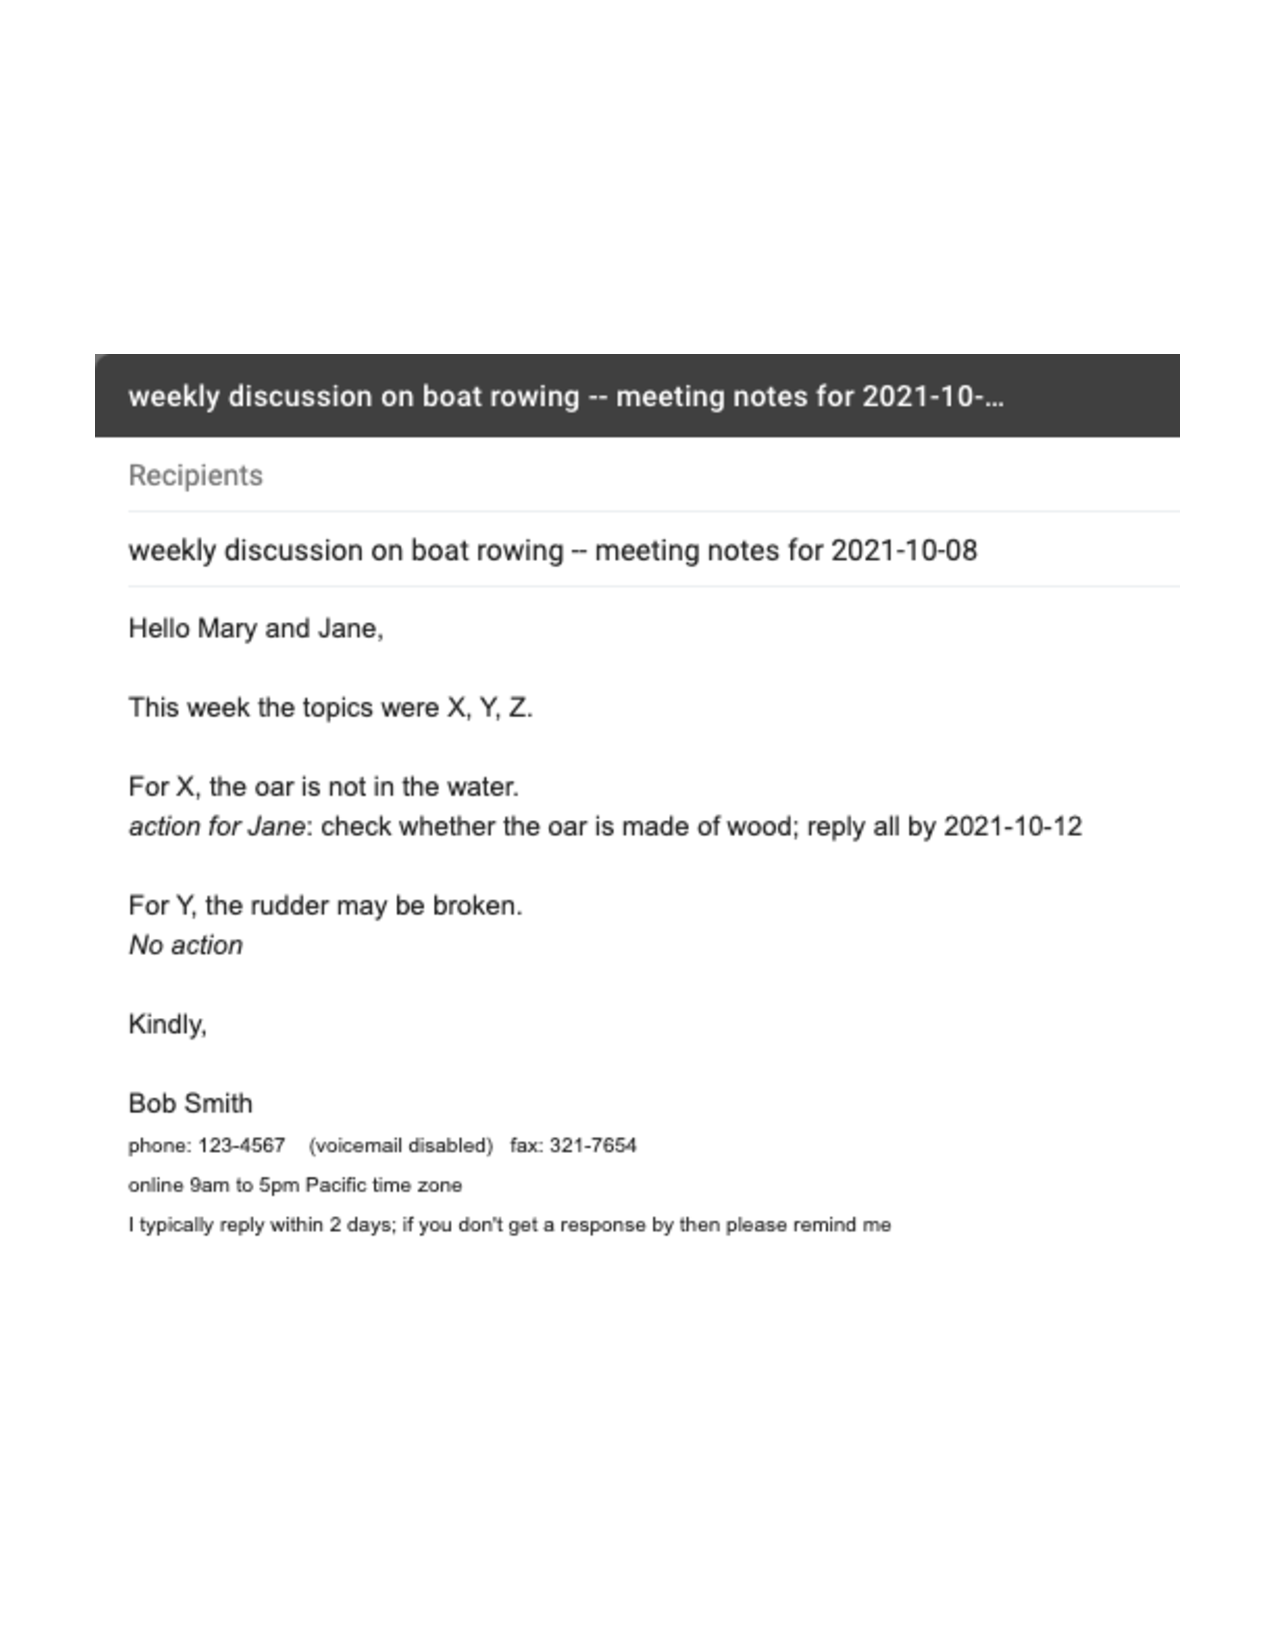
\includegraphics[width=1\textwidth]{images/email_meeting_notes.pdf}
\caption{Who has what action due when?}
\label{fig:email_meeting_notes}
\end{figure}

Computer commands should be distinct separate fixed-width font. This distinguishes the text from the rest of the narrative. 


\begin{figure}
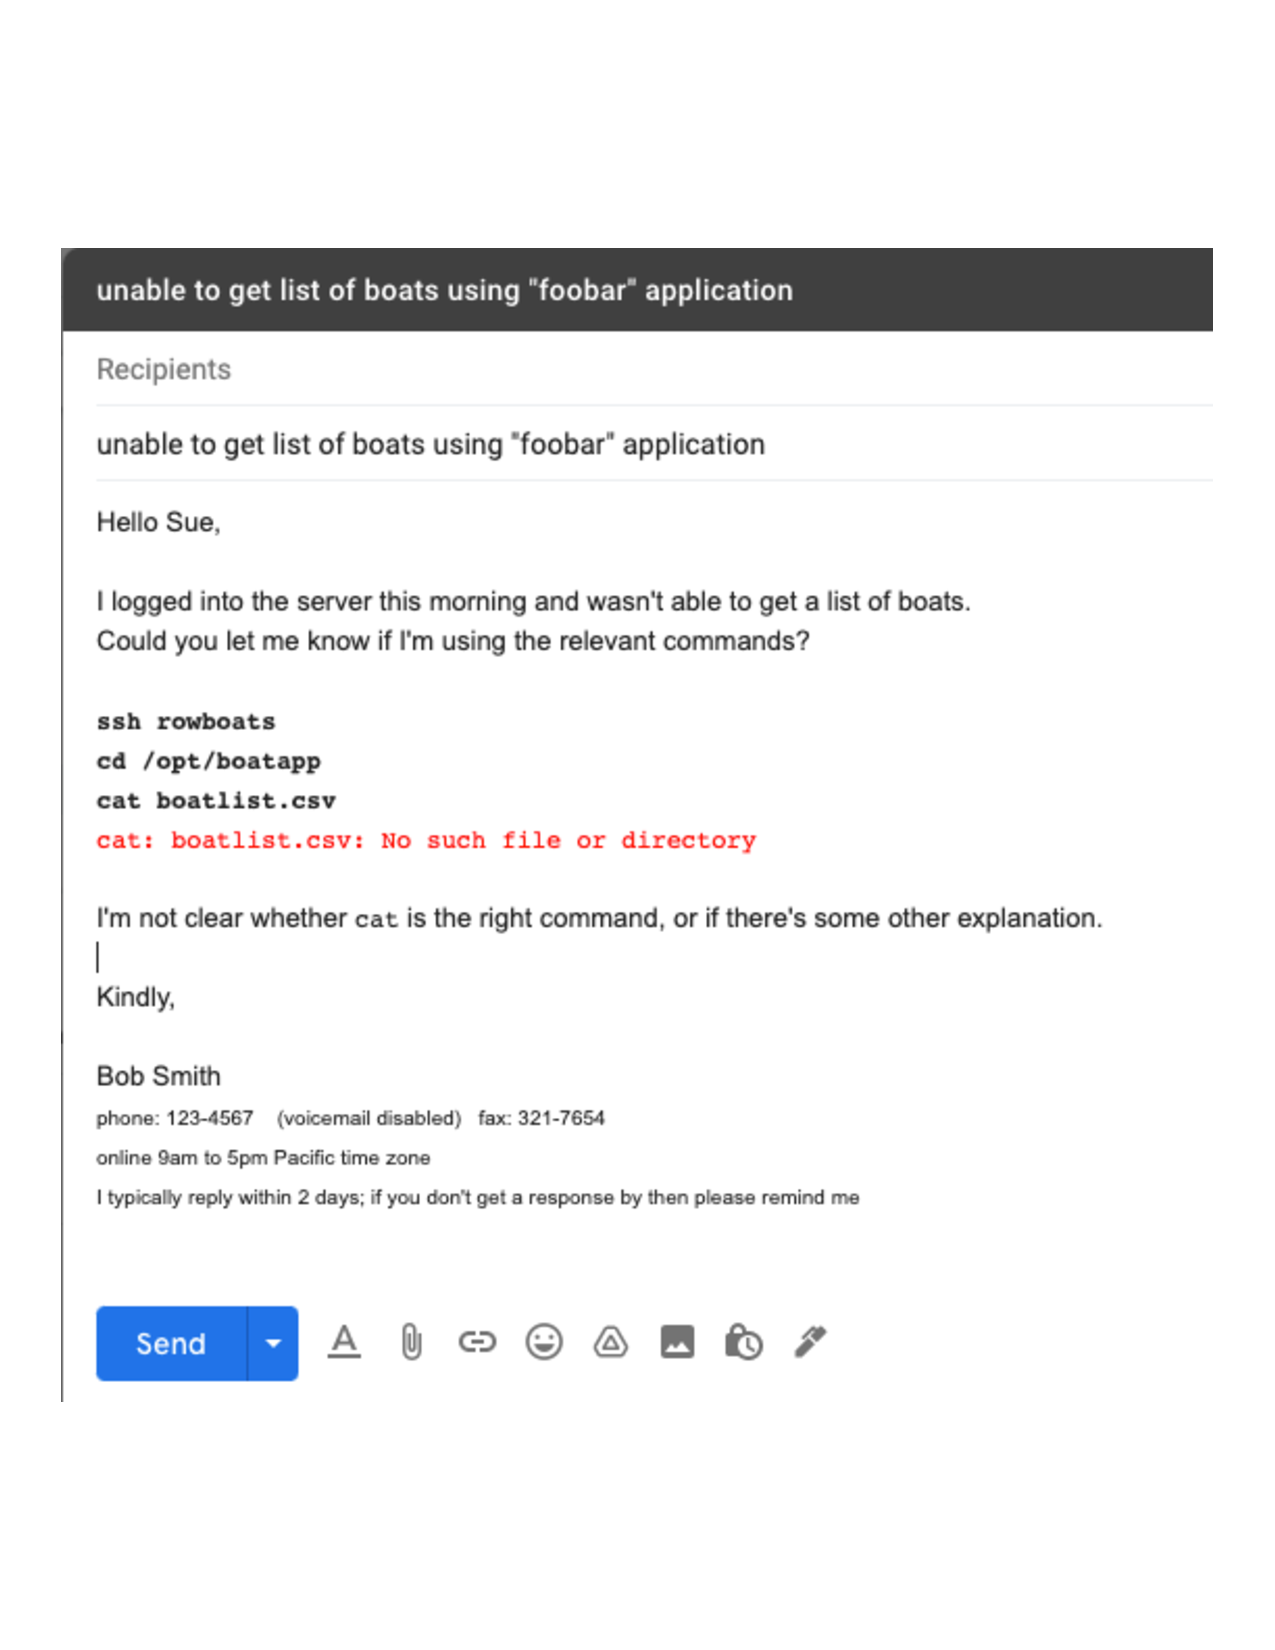
\includegraphics[width=1\textwidth]{images/email_computer_font.pdf}
\caption{The computer commands use fixed width font. The author distinguished input from output through the use of bold vs non-bold respectively. The author highlighted the error message using red. Inline text like cat in the last line is also fixed with.}
\label{fig:email_computer_font}
\end{figure}

References to documents include a direct full path.

If referring to a previous separate thread, include the subject and the date+time that email was sent

For bullet points, explicitly specify that items are joined by one of the following: OR, XOR, AND

If you have an unordered list, explicitly state that order is irrelevant.

If you have a sequence of steps, number them appropriately and indicate which steps are required versus optional

Use visual sketches to illustrate concepts rather than always relying on text. Don't use pictures all the time, and don't have too many pictures in an email. 

Know how to both embed pictures inline and how to attach files and when to use which. 
Email replies should preferentially be at the top of the thread. 
If replying to multiple points in the previous email, embed replies inline, mark the distinction, and highlight the authorship. 

\begin{figure}
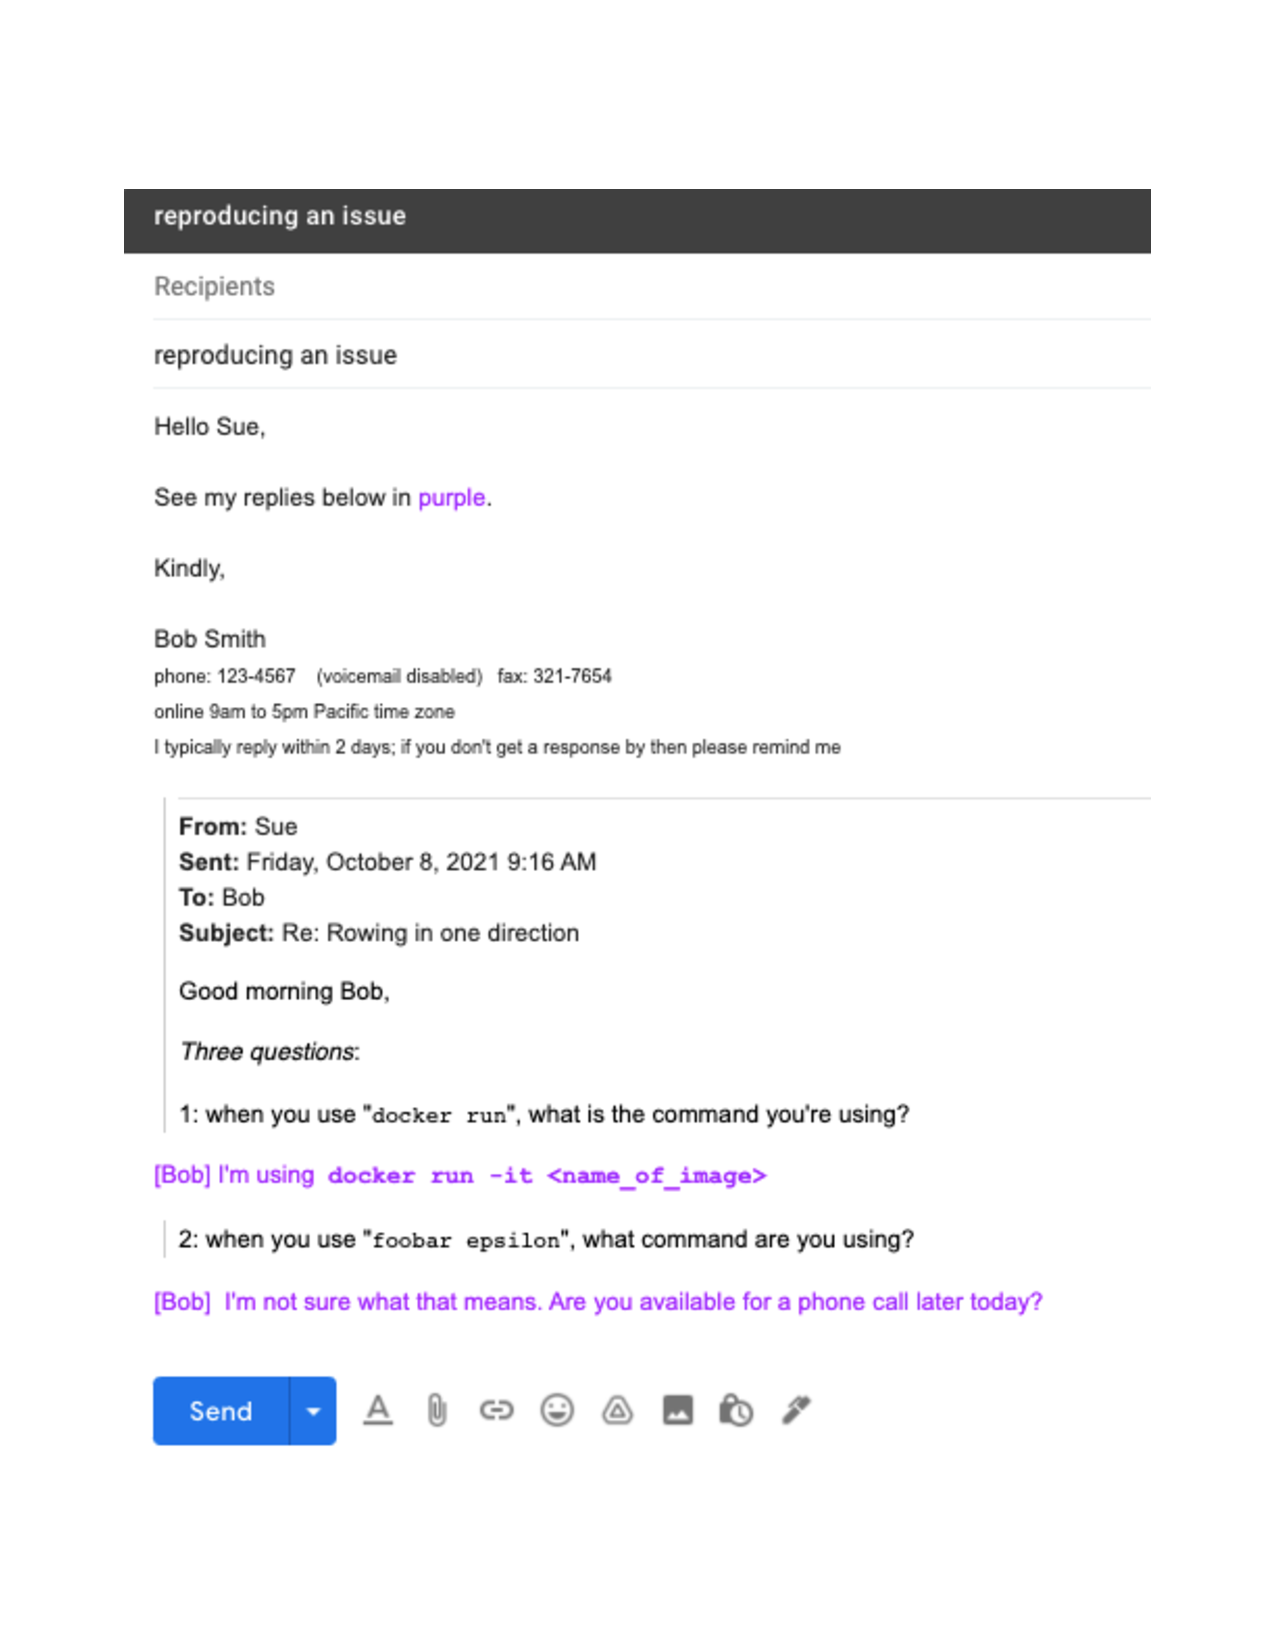
\includegraphics[width=1\textwidth]{images/email_reply.pdf}
\caption{Bob's reply to Sue's questions. The third question is not shown in this illustration.}
\label{fig:email_reply}
\end{figure}

If replying inline, explicitly state that at the top of the thread.

The email trilemma is to balance the amount of detail against providing sufficient context and being concise. 

If the email requires a \href{https://en.wikipedia.org/wiki/BLUF_(communication)}{B.L.U.F} or \href{https://en.wikipedia.org/wiki/Wikipedia:Too_long;_didn\%27t_read}{tl;dr} or summary, then it's too long. Inclusion of a BLUF or tl;dr risks resulting in the reader skipping the content. 

Emails convey both emotional tone and facts. Your intent is practically irrelevant; the reader's perception is paramount. 

Every email should have a purpose. What are you asking the recipient to do? How do you want them to feel? How should they respond?

When replying, starting your email with an expression of gratitude for the work the recipient has done so far sets a positive tone by acknowledging their investment.

